\documentclass{beamer}
\usetheme{Madrid}
\title{Hamiltonian Circuit}
\author[Rafi and Mrittunjay]{Rakibul Islam \inst{1}\\
Mrittunjay Roy \inst{1}}
\institute[CSE,BUET]{
\inst{1}
Department of CSE,BUET\\
}
\date{\today}
\begin{document}
\begin{frame}
\titlepage
\end{frame}
\begin{frame}
\frametitle{What is Hamitonian Cycle?}
\begin{columns}
\column{0.7\textwidth}
\begin{block}{Cycle}
In graph theory, a cycle is a path of edges and vertices wherein a vertex is reachable from itself.
\end{block}
\begin{block}{Hamiltonian Circuit}
A Hamiltonian circuit,also known as Hamiltonian cycle,  is a cycle that visits each vertex exactly once (except for the vertex that is both the start and end, which is visited twice).
\end{block}
\column{0.3\textwidth}
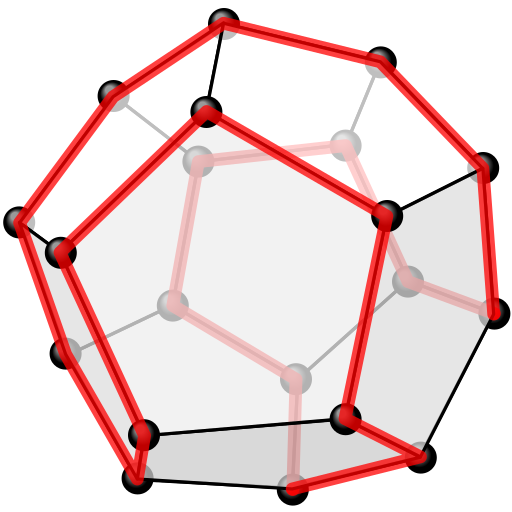
\includegraphics[scale=.2]{hamcycle.png}
\end{columns}
\end{frame}

\begin{frame}
\frametitle{History}
\begin{itemize}
\onslide<1,7>{
\setbeamercovered{transparent}
\item The Hamiltonian cycle is named after Sir William Rowan Hamilton.
}
\onslide<2,7>{
\setbeamercovered{transparent}
\item He devised a puzzle in which such a path along the polyhedron edges of an dodecahedron was sought (the Icosian game).
}
\onslide<3,7>{
\setbeamercovered{transparent}
\item The Icosian Game was invented in 1857.
}
\onslide<4,7>{
\setbeamercovered{transparent}
\item The Icosian game is the problem of finding a Hamiltonian cycle along the edges of an dodecahedron, i.e., a path such that every vertex is visited a single time, no edge is visited twice, and the ending point is the same as the starting point.
}
\onslide<5,7>{
\setbeamercovered{transparent}
\item Hamilton sold it to a London game dealer in 1859 for 25 pounds.
}
\onslide<6,7>{
\setbeamercovered{transparent}
\item the game was subsequently marketed in Europe in a number of forms (Gardner 1957).
}
\end{itemize}
\end{frame}
\begin{frame}
\frametitle{Hamiltonian Graph}
\onslide<1>{\begin{definition}
 A graph that contains a Hamiltonian cycle is called a Hamiltonian graph.
\end{definition}
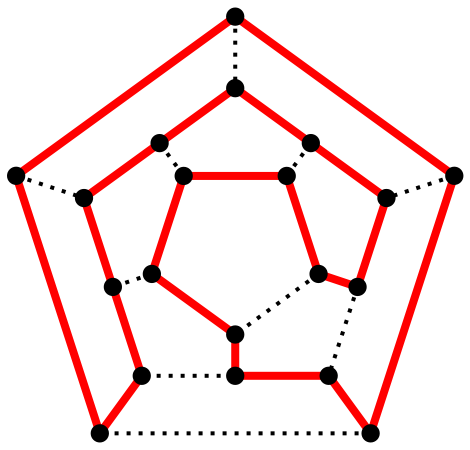
\includegraphics[scale=.16]{hamcycle1.png}
\centering
}

\onslide<2->{\textcolor<2->{red}{Does every graph has a Hamiltonian Cycle?}}

\onslide<3->{
\begin{columns}
\column{0.7\textwidth}
\begin{alertblock}{Caution}
Not every graph is a Hamiltonian graph.
\end{alertblock}
\column{0.3\textwidth}
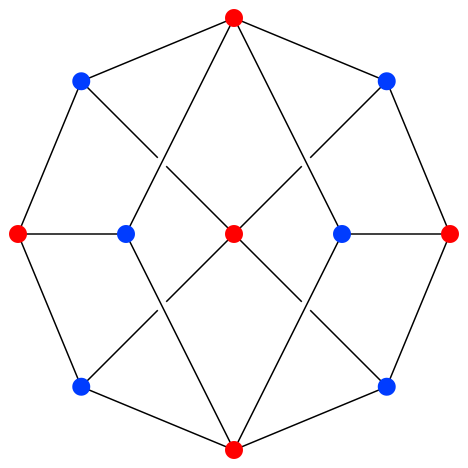
\includegraphics[scale=.15]{Notham.png}
\end{columns}

}
\end{frame}

\begin{frame}
\frametitle{Finding Hamiltonian Cycle in Graphs}
\begin{itemize}
    \item In general, the problem of finding a Hamiltonian cycle is NP-complete.
    \pause
    \item So,the only known way to determine whether a given general graph has a Hamiltonian cycle is to undertake an exhaustive search.
\end{itemize}
\end{frame}
\begin{frame}
\frametitle{Algoritms}
\onslide<1,4>{\begin{block}{Algorithm of Martello}
    A brute force algorithm.Tests n! different sequences of vertices that might be Hamiltonian paths in a given n-vertex graph.
\end{block}}
   \onslide<2,4>{
\begin{block}{Algorithm of Rubin}
    A search procedure that divides the edges of the graph into three classes: those that must be in the path, those that cannot be in the path, and undecided. As the search proceeds, a set of decision rules classifies the undecided edges, and determines whether to halt or continue the search.
\end{block}
}
\onslide<3,4>{
\begin{block}{Algorithm of Bellman,Held and Karp}
    A dynamic programming algorithm that can be used to solve the problem in time O($n^2$ $2^n$).
\end{block}
}
\end{frame}
\begin{frame}
\frametitle{Algoritms}
    \centering
   
\includegraphics[scale=.5]{th.png}
   \centering
   \huge Any Questions?

\end{frame}
\end{document}
